\documentclass[a4paper,10pt]{report}
\usepackage{xunicode}
\usepackage{xltxtra}
\usepackage{color}
\usepackage{enumerate}
\usepackage[top=1.5cm, bottom=1.5cm, left=1.5cm, right=1.5cm]{geometry}
\usepackage{url}
\usepackage{hyperref}

\usepackage{minted}
\definecolor{frame_color}{gray}{0.70}
\addtolength\fboxsep{0.2cm}
\usemintedstyle{trac}
\newminted[code]{haskell}{xleftmargin=1cm, samepage=true}

\usepackage{fancyvrb}
%\DefineVerbatimEnvironment{code}{Verbatim}{frame=single, framerule=0.5mm, fontsize=\small, formatcom=\color{blue}}
%\DefineVerbatimEnvironment{example}{Verbatim}{}
\DefineShortVerb{\|}

\newcommand{\includeSource}[1]{
  \inputminted[frame=single, rulecolor=\color{frame_color}]{haskell}{#1}
}

\newcommand{\includeHaskell}[3]{
  The source code for this section is contained in \path{#1}.
  \begin{listing}[H]
  \inputminted[frame=single, rulecolor=\color{frame_color}]{haskell}{#1}
  \caption{#3}
  \label{lst:{#2}}
  \end{listing}
}

\title{Créatúr Tutorial}
\author{Amy de Buitl\'eir\\
        Email: amy@nualeargais.ie}

\begin{document}

\maketitle

\tableofcontents

\chapter{Overview of Créatúr}

Créatúr\footnote{\emph{Créatúr} (pronounced kray-toor) is an irish word 
meaning animal, creature, or unfortunate person.} 
is a software framework for automating experiments
with artificial life (ALife). 
It provides a daemon which ensures that each agent gets its turn 
to use the CPU. 
You can use other applications on the computer at the same time
without fear of interfering with experiments; they
will run normally (although perhaps more slowly).
Créatúr also provides a library of modules to help you implement your own 
ALife species.
Even if you aren't using the Créatúr framework, you may find some of these
modules useful.

\chapter{Getting started}
\label{sec:install}

The instructions below should work on Linux, Windows, or OSX.

\begin{enumerate}
\item Make sure you've installed the Haskell platform. You can get it from
\url{http://hackage.haskell.org/platform/}.

\item At the command prompt, type |cabal install creatur|.
This will install the Créatúr framework.

\item Download |creatur-examples-master.zip| from
\url{https://github.com/mhwombat/creatur-examples/archive/master.zip}.
This contains the examples used in this tutorial.

\item Unzip the file you just downloaded (|creatur-examples-master.zip|).
This will create a directory called \path{creatur-examples-master}.

\item At the command prompt, go to the directory you just created.
(|cd creatur-examples-master|).

\item Build and install the examples by typing |cabal install|.
\end {enumerate}

If you've never used Haskell before, I recommend the following
books.
The complete content of both books is freely available online,
so try both and see which one best suits your learning style.
As suggested by the title, \emph{Real World Haskell} teaches
Haskell using a series of practical examples.
\emph{Learn You a Haskell} is presented with a great deal of humour,
and may give you a deeper understanding of functional programming
concepts.

\begin{itemize}
\item Learn You a Haskell for Great Good!: A Beginner's Guide \\
Miran Lipovaca \\
ISBN-13: 978-1593272838 \\
\url{http://learnyouahaskell.com/}

\item Real World Haskell \\
Bryan O'Sullivan, Don Stewart, and John Goerzen \\
ISBN-13: 978-0596514983 \\
\url{http://book.realworldhaskell.org/}
\end {itemize}


The Haskell community is very friendly and welcoming to newbies.
Two good places to ask questions are 
the beginners@haskell.org mailing list
(see \url{http://www.haskell.org/haskellwiki/Mailing_lists} 
for more information)
and Stack Overflow \url{http://stackoverflow.com/questions/tagged/haskell}.

The API documentation for Créatúr is available at 
\url{http://hackage.haskell.org/package/creatur}.

\chapter{The main daemon loop}
\label{sec:daemon}

The daemon clock is a simple counter used to schedule events.
At each tick of the clock, the daemon:

\begin{enumerate}
\item Reads the current list of agents, which are stored as separate files in
the current directory.
\item Queues the agents in random order.
\item Processes the queue, giving each agent an opportunity
to use the CPU by invoking a user-supplied function.
\item Increments the daemon clock.
\end {enumerate}

A different random order is used at each clock tick
so that no agent has an unfair advantage.
(If agents were always processed in the same order, 
agents near the end of the list might, for example, find that that the 
best food has already been eaten or that the desirable mating
partners are already taken.)

\chapter{Overview of the process}

The steps for using Créatúr to create and run an ALife experiment
are listed below.

\begin{enumerate}
\item Create one or more ALife species
\item Generate an initial population
\item Configure a daemon
\item Build and run the universe
\end {enumerate}

\chapter{A very simple species}
\label{sec:rock}

In this part of the tutorial, we create and run a universe
with a very simple species.
This will introduce you to the basics of the Créatúr framework.

\section{Create a species}
\label{sec:species1}

We'll only use one species in this example, and it will be a very simple 
species called |Rock|.
Rocks don't reproduce, so we don't need to worry about genetics.

A complete listing of the source code discussed here is provided on 
page \pageref{code:rock}.
We'll discuss the main points here.
The |DeriveGeneric| pragma activates support for generics
(available beginning with GHC 7.2 or the Haskell Platform 2012.4.0.0),
which allows some code to be generated automatically for us.

\begin{code}
{-# LANGUAGE DeriveGeneric #-}
\end{code} 

|Rock|s have a unique ID, and a counter. 
We will use the counter to demonstrate that the Créatúr
framework persists (``remembers'') the state of the rock
from one run to the next.

\begin{code}
data Rock = Rock String Int deriving (Show, Generic)
\end{code} 

All agents used in the Créatúr framework must be an instance of
|Serialize|, which ensures that they can be written to and read from a
database or file system.
Notice that we do not need to write |put| and |get| functions.
Deriving |Generic| instructs Haskell to generate them for us.

\begin{code}
instance Serialize Rock
\end{code} 

All species used in the Créatúr framework must be an instance of 
|ALife.Creatur.Agent|,
which requires us to implement two functions: |agentId| and |isAlive|.
The function |agentId| returns a unique identifier for this agent.
The function |isAlive| indicates whether the agent is currently alive
(if it is not alive, it would automatically be archived).
Since rocks never die, this function can simply return |True|.

\begin{code}
instance Agent Rock where
  agentId (Rock name _) = name
  isAlive _ = True
\end{code} 

Making |Rock| an instance of |ALife.Creatur.Database.Record|
allows us to store agents and retrieve them from the file system.
A record needs a unique identifier;
we can use |agentId| for this purpose.

\begin{code}
instance Record Rock where key = agentId
\end{code} 

Finally, we need to write the function that will be
invoked by the daemon when it is the agent's turn to use the CPU.
This function is passed as a configuration parameter to the daemon,
as will be seen in Section \ref{sec:daemon1}.
This example is quite simple;
it merely writes a message to the log file
and returns a new version of the rock, with an updated counter.
However, this is where your agents get a chance to eat, mate, 
and do whatever else they need to do.
We'll see a more typical implementation in Section
\ref{sec:species2}.

\begin{code}
run :: Rock -> StateT (SimpleUniverse Rock) IO Rock
run (Rock name k) = do
  writeToLog $ name ++ "'s turn. counter=" ++ show k 
  return $ Rock name (k+1)
\end{code}

The type signature of |run| is explained in Section \ref{sec:daemon1}.
The complete code listing is below.
\label{code:rock}
\includeSource{src/Tutorial/Chapter5/Rock.hs}



\section{Generate an initial population}
\label{sec:pop1}

We will create our first population in a directory called |Chapter5|.
In |main|, we initialise the |chapter5| directory, create two rocks,
and write them to the directory.
The parameters to the |mkSimpleUniverse| command specify the name of the universe,
and the path to the directory that contains it.
When a log file reaches the maximum size, it is closed and a new log file is started.
\includeSource{src/Tutorial/Chapter5/GeneratePopulation.hs}



The procedure for running this program will be described in Section 
\ref{sec:run1}.

\section{Configure a daemon}
\label{sec:daemon1}


The module \path{ALife.Creatur.Universe.Task} provides some tasks
that you can use with the daemon.
These tasks handle reading and writing agents,
which reduces the amount of code you need to write.
(It's also easy to write your own tasks, using those in 
\path{ALife.Creatur.Universe.Task} as a guide.)
The simplest task has the type signature:

\begin{code}
runNoninteractingAgents
  :: (Universe u, Serialize (Agent u))
    => AgentProgram u -> SummaryProgram u -> StateT u IO ()
\end{code}

That signature looks complex, but essentially it means that if you
supply an |AgentProgram|, it will run it for you.
So what type signature must your |AgentProgram| have?
Here's the definition.

\begin{code}
type AgentProgram u = Agent u -> StateT u IO (Agent u)
\end{code}

This is the signature for an agent that doesn't interact with other
agents.
The input parameter is the agent whose turn it is to use the CPU.
The program must return the agent (which may have been modified).
The universe will then automatically be updated with these changes.
We will use the |run| function in \path{Tutorial.Chapter5.Rock}
(discussed in Section \ref{sec:species1}) as our |AgentProgram|.
Its type signature is shown below.

\begin{code}
run :: Rock -> StateT (SimpleUniverse a) IO Rock
\end{code}

|SimpleUniverse a| provides the logging, clock, and agent naming
functionality we need.
So the type signature of |run| is consistent with |AgentProgram|.
The program below configures and launches the daemon.

\includeSource{src/Tutorial/Chapter5/Daemon.hs}



\section{Build and run the example}
\label{sec:run1}


Here is the listing of |creatur-examples.cabal|.
\verbatiminput{creatur-examples.cabal}

\begin{enumerate}
\item If you haven't already done so, follow the instructions in Chapter
\ref{sec:install}.
\item Create the initial population by running |chapter5-init|.
\item Start the daemon with the command |sudo chapter5-daemon start|.
\item Stop the daemon with the command |sudo chapter5-daemon stop|.
(Stopping the daemon may take a few seconds.)
\end{enumerate}

Log messages are sent to |chapter5/log/Chapter5.log|.
Examine that file and notice that the counter is counting up for both rocks.
If you stop the daemon and restart it, it will pick up where it left off
\footnote{When the stop command is received, the daemon will attempt
to finish the processing for the current clock tick.
Depending on the processor speed and the number of agents in the population,
it may not finish before the hard kill which is issued three seconds later.
The database or file system is not updated until an agent's turn at the CPU 
is complete, so any partial results are discarded.
If the daemon terminates while an agent is running,
the effect is that the current agent, and all others after it in the queue,
miss their turn at the CPU.
However, even frequent restarting of the daemon
is unlikely to cause CPU starvation for any particular agent.
The random order in which agents are processed spreads the impact
over the population.}, preserving the value of the 
counter between runs.

A sample extract from the log file is shown below.
The first field is the system clock time.
The second field is the daemon clock time.
The third field is the log message.
Note that in clock tick |0|, |Rocky| gets to use the CPU before |Rocky|,
while in clock tick |3|, |Roxie| goes first.
This demonstrates the randomisation discussed in section \ref{sec:daemon}.

\begin{verbatim}
130121121233+0000       Starting
130121121233+0000       0       Rocky's counter is 42
130121121233+0000       0       Roxie's counter is 99
130121121233+0000       1       Rocky's counter is 43
130121121233+0000       1       Roxie's counter is 100
130121121233+0000       2       Roxie's counter is 101
130121121233+0000       2       Rocky's counter is 44
130121121233+0000       3       Roxie's counter is 102
130121121233+0000       3       Rocky's counter is 45
130121121234+0000       4       Rocky's counter is 46
130121121234+0000       4       Roxie's counter is 103
\end{verbatim}

\chapter{Recombination}
\label{sec:recombination}

When agents that reproduce, the offspring will inherit a mixture of
genetic information from both parents.
Here are two scenarios that could be used, although there are other
possibilities.

\begin{enumerate}
\item Your agents use \emph{asexual} reproduction.
Each agent has a \emph{single} sequence of genetic information.
When two agents mate, their genes are shuffled to produce
two \emph{new} sequences.
You can create two children from these sequences,
or discard one sequence and create a child with the remaining sequence.
\item Your agents use \emph{sexual} reproduction.
Each agent has \emph{two} sequences of genetic information.
When two agents mate, each agent contributes \emph{one}
sequence to the child.
A parent's two sequences are shuffled to produce two \emph{new}
sequences.
One of the sequences is discarded; the other sequence becomes
that parent's contribution to the child's genome.
The same process occurs with the other parent's genome.
The two sequences (one from each parent) are combined to create the 
child's genome.
This is analogous to the production of a \emph{gamete} (ovum or sperm) 
in biology.
\end{enumerate}

Both scenarios involve shuffling a pair of sequences to produce two new
pairs, and possibly discarding one of the sequences.
In addition, you may wish to allow occasional random mutations.
The Créatúr framework provides the 
several operations for this purpose, in the
\path{ALife.Creatur.Genetics.Recombination} package.
These operations can be applied (multiple times)
with specified probabilities
and combined in various ways.
Two common operations, \emph{crossover} and \emph{cut-and-splice},
are illustrated below.
In crossover, a single crossover point is chosen.
All data beyond that point is swapped between strings.
In cut-and-splice, two points are chosen, one on each string.
This generally results in two strings of unequal length.

\begin{figure}[hbtp]
 \centering
 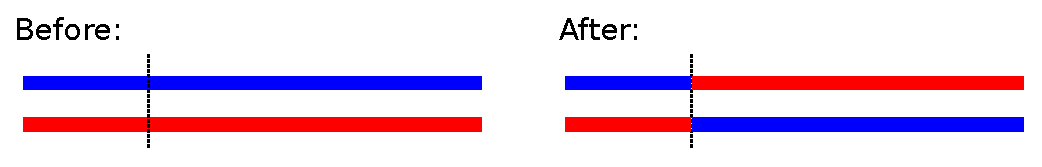
\includegraphics[scale=0.7,keepaspectratio=true]{./images/crossover.eps}
  \caption{Crossover}
  \label{fig:crossover}
\end{figure}

\begin{figure}[hbtp]
 \centering
 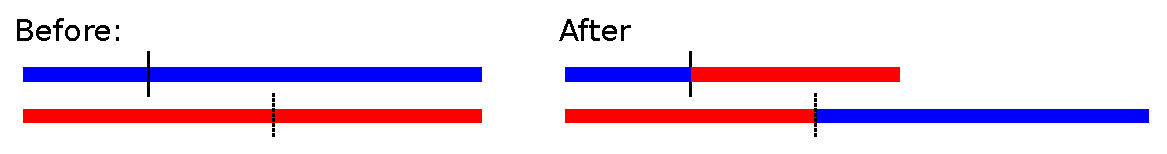
\includegraphics[scale=0.7,keepaspectratio=true]{./images/cut-and-splice.eps}
  \caption{Cut-and-splice}
  \label{fig:cut-and-splice}
\end{figure}

Here's a sample program that might be used to shuffle two
sequences of genetic material.

\label{code:recombination}
\begin{code}
    withProbability 0.1 randomCrossover (xs, ys) >>=
    withProbability 0.01 randomCutAndSplice >>=
    withProbability 0.001 mutatePairedLists >>=
    randomOneOfPair
\end{code} 

To understand how this program works,
let's walk through a simple example.
Suppose this program acted on the following pair of sequences:
\begin{code}
([A,A,A,A,A,A,A,A,A,A],[C,C,C,C,C,C,C,C,C,C])
\end{code} 
The |randomCrossover| function \emph{might} perform a simple crossover,
perhaps resulting in:
\begin{code}
([A,A,A,A,A,A,A,C,C,C],[C,C,C,C,C,C,C,A,A,A])
\end{code} 
The|randomCutAndSplice| function \emph{might} then perform a cut-and-splice, perhaps
resulting in:
\begin{code}
([A,A,A,A,C,A,A,A],[C,C,C,C,C,C,A,A,A,C,C,C])
\end{code} 
The |mutatePairedLists| function \emph{might} then mutate one or both sequences, perhaps
resulting in
\begin{code}
([T,A,A,A,C,A,A,A],[C,C,C,C,C,C,A,A,C,C,C,C])
\end{code} 
The numbers 0.1, 0.01, and 0.001 control the likelihood of each
of the three operations occurring.
After the first three operations, we have two new sequences.
In this example, we only want one of the sequences,
so the final line randomly chooses one.

To perform more than one crossover, the operation can simply be repeated
as shown below.

\begin{code}
    withProbability 0.1 randomCrossover (xs, ys) >>=
    withProbability 0.08 randomCrossover (xs, ys) >>=
    . . .
\end{code} 

Alternatively, we can choose the number of crossover operations at 
random. The function |repeatWithProbability| performs an operation a
random number of times, such that the probability of repeating the
operation |n| times is $p^n$.

\begin{code}
    repeatWithProbability 0.1 randomCrossover (xs, ys) >>=
    . . .
\end{code} 

Other recombination operators are also available.
Consult the documentation of \path{ALife.Creatur.Genetics.Recombination}
for more information.

\chapter{Asexual reproduction}
\label{sec:plant}

In this part of the tutorial, we create a species with the
ability to reproduce asexually.

\section{Create a species}
\label{sec:species2}

The species used in this example is called |Plant|.
Each |Plant| has a unique ID, a flower colour,
an energy level, and some genetic information.
(A complete listing of the source code discussed here is provided on 
page \pageref{code:plant}.)

\begin{code}
data Plant = Plant
  { 
    plantName :: String,
    plantFlowerColour :: FlowerColour,
    plantEnergy :: Int,
    plantGenome :: Sequence
  } deriving (Show, Generic)
\end{code} 

As with |Rock|s, the type |Plant| will be an instance of 
the |Serialize|, |Agent| and |Record| classes.
Our plants will stay alive until all of their energy is gone.

\begin{code}
instance Serialize Plant

instance Agent Plant where
  agentId = plantName
  isAlive plant = plantEnergy plant > 0

instance Record Plant where key = agentId
\end{code} 

We'll have a choice of flower colours.
\begin{code}
data FlowerColour = Red | Orange | Yellow | Violet | Blue
  deriving (Show, Eq, Generic, Enum, Bounded)
\end{code} 

In order for |Plant| to be an instance of |Serialize|,
any type that it uses must also be an instance.
So we make |FlowerColour| be an instance of |Serialize|.

\begin{code}
instance Serialize FlowerColour
\end{code} 

We need a way to encode the plant genes into DNA-like sequences that can
be shuffled, or even mutated, during reproduction.
We'll encode the genes as sequences of |Bool|s.
We could write our own coding scheme, but \path{ALife.Creatur.Genetics.Code.BRGCBool}
provides a scheme for us, using a class called |Gene|.
The |Gene| class provides the method |put|, which encodes a gene and writes it to a sequence,
and the method |get|, which reads and decodes the first gene in a sequence.
By making |FlowerColour| an instance of |Gene|, 
|FlowerColour| will be encoded as a string of boolean values using a \emph{Gray code}.
A Gray code maps values to codes in a way that guarantees that the codes
for two consecutive values will differ by only one bit. This feature
is useful for encoding genes because the result
of a crossover operation will be similar to the inputs. 
This helps to
ensure that offspring are similar to their parents, as any radical
changes from one generation to the next are the result of mutation
alone.

When the genes of an agent have a small set of possible values,
it is practical to store their genetic information as a string of |Bool|s.
(If an agent has genes with a larger number of possible values,
it may be better to store their genetic information as a string of numbers.
Créatúr also provides \path{ALife.Creatur.Genetics.Code.BRGCWord8},
which encodes the genes using a Gray code, but stores them using a string of |Word8|s.
Since |BRGCWord8| provides most of the same functions as |BRGCBool|,
all we need to do to make |Plant| use |Word8|s is to import |BRGCWord8|
instead of |BRGCBool|.)
We'll see an example of this in Section \ref{sec:species4}.

\begin{code}
instance Genetic FlowerColour
\end{code} 

To support reproduction, we need a way to build a plant from its genome.
First, each plant needs a copy of its genome in order to produce offspring;
we'll use the |copy| method to obtain this.
Next, we determine the colour of the bug.
We could use the method |get| in the class |Gene|, 
which returns a |Maybe| value containing the next gene in a sequence.
However, our sequence of |Bool|s may not
be a valid code for a colour, in which case the call to |get|
would return |Nothing|.
In this example, we will create a plant no matter what errors there are in 
the genome, so we will use |getWithDefault|, using |Red| as the default value.
(Alternatively, we could treat the mutation as non-viable,
and not create the offspring.
We'll see an example of that in Section \ref{sec:species4}.
All plants start life with an energy of |10|.
        
\begin{code}
buildPlant :: String -> Reader (Maybe Plant)
buildPlant name = do
  g <- copy
  colour <- getWithDefault Red
  return . Just $ Plant name colour 10 g
\end{code} 

We need a way to mate two plants and produce some offspring.
We can do this by implementing the |Reproductive| class in 
\path{ALife.Creatur.Genetics.Reproduction.Asexual}.
This class requires us to implement the following:
\begin{enumerate}
\item A type called |Base|, which specifies the type used to encode
genes for this species. Recall that we've used |Bool|s for this purpose.
\item A method called |recombine| which shuffles (and maybe mutates) the
 parent's genes to produce the offspring.
\item A method called |build| which creates the offspring.
We can call the |read| method in the |Reproductive| class,
supplying the |buildPlant| method as an argument.
\end {enumerate}

\begin{code}
instance Reproductive Plant where
  type Base Plant = Sequence
  recombine a b = 
    withProbability 0.1 randomCrossover (plantGenome a, plantGenome b) >>=
    withProbability 0.01 randomCutAndSplice >>=
    withProbability 0.001 mutatePairedLists >>=
    randomOneOfPair
  build name = runReader (buildPlant name)
\end{code} 

The implementation for |recombine| uses the sample recombination
program discussed on page \pageref{code:recombination}.
Next, we write the function |run|, 
which is invoked when it is the agent's turn to use the CPU.
Because our plants need to interact in order to mate,
when we write the daemon (in Section \ref{sec:daemon2}) we will use
|runInteractingAgents| instead of |runNoninteractingAgents|.
This requires a different type signature for |run| than we used for
rocks.
The type signature we need is

\begin{code}
type AgentsProgram c l d n x a = 
  [a] -> StateT (Universe c l d n x a) IO [a]
\end{code} 

The input parameter is a list of agents. 
The first agent in the list is the agent whose turn it is to use the 
CPU.
The rest of the list contains agents it could interact with.
(We only need to use the first two elements of this list.)
Finally, the program must return a list of agents that it has modified.

The function |run| is invoked when it is the agent's turn to use the CPU.
It takes a list of all agents in the population, with the current agent at the head of the list.
It returns a list of agents that have been created or modified during the turn.
In this implementation, |run| ``mates'' two plants and takes away one unit of energy 
to represent the energy cost of reproduction
(otherwise the plants would live forever).

\begin{code}
run :: [Plant] -> StateT (SimpleUniverse Plant) IO [Plant]
run (me:other:_) = do
  name <- genName
  (Just baby) <- liftIO $ evalRandIO (makeOffspring me other name)
  writeToLog $ 
    plantName me ++ " and " ++ plantName other ++
      " gave birth to " ++ name ++ ", with " ++ 
       show (plantFlowerColour baby) ++ " flowers"
  return [deductMatingEnergy me, deductMatingEnergy other, baby]
run x = return x -- need two agents to mate
\end{code}

The complete code listing is below.
\label{code:plant}
\includeSource{src/Tutorial/Chapter7/Plant.hs}



\section{Generate an initial population}
\label{sec:pop2}

We will create the next population in a directory called |chapter7|.
In |main|, we initialise the |chapter7| directory, create three 
|Plant|s, and write them to the directory.
The initial population only contains plants with red, yellow, 
or violet flowers.
Eventually, plants with orange or blue flowers might appear, but only
as the result of mutation.
(In Section \ref{sec:pop4}, we introduce a different technique for creating
an initial population, using random genetic sequences.)
The complete code listing is below.

\includeSource{src/Tutorial/Chapter7/GeneratePopulation.hs}



\section{Configure a daemon}
\label{sec:daemon2}

The program below configures and launches the daemon.

\includeSource{src/Tutorial/Chapter7/Daemon.hs}



\section{Build and run the example}
\label{sec:run2}

\begin{enumerate}
\item If you haven't already done so, follow the instructions in Chapter 
\ref{sec:install}.
\item Create the initial population by running |chapter7-init|.
\item Start/stop/restart the daemon with the command
\UndefineShortVerb{\|}
\DefineShortVerb{\+}
+sudo chapter7-daemon start|stop|restart+.
\UndefineShortVerb{\+}
\DefineShortVerb{\|}
(Stopping the daemon may take a few seconds.)
\end{enumerate}

Log messages are sent to |chapter7/log/Chapter7.log|.

A sample extract from the log file is shown below.
To conserve space, the timestamps have been omitted.
From this, you can see that the first mating (between |Rose| and |Sunny|)
occurs at time 0.
The offspring, |Chapter7_1|, gets its first CPU turn at time 1.

\begin{verbatim}
Starting
0       Vi and Rose gave birth to Chapter7_1, with Red flowers
0       Rose and Vi gave birth to Chapter7_2, with Violet flowers
0       Sunny and Rose gave birth to Chapter7_3, with Red flowers
1       Chapter7_1 and Sunny gave birth to Chapter7_4, with Yellow flowers
1       Rose and Vi gave birth to Chapter7_5, with Violet flowers
1       Chapter7_3 and Chapter7_2 gave birth to Chapter7_6, with Red flowers
1       Chapter7_2 and Sunny gave birth to Chapter7_7, with Violet flowers
1       Vi and Chapter7_7 gave birth to Chapter7_8, with Violet flowers
1       Sunny and Chapter7_8 gave birth to Chapter7_9, with Yellow flowers
2       Chapter7_4 and Rose gave birth to Chapter7_10, with Yellow flowers
2       Chapter7_7 and Chapter7_6 gave birth to Chapter7_11, with Violet flowers
2       Chapter7_6 and Rose gave birth to Chapter7_12, with Red flowers
2       Chapter7_5 and Chapter7_10 gave birth to Chapter7_13, with Violet flowers
2       Chapter7_3 and Chapter7_7 gave birth to Chapter7_14, with Red flowers
2       Chapter7_8 and Chapter7_14 gave birth to Chapter7_15, with Red flowers
2       Rose and Chapter7_14 gave birth to Chapter7_16, with Red flowers
2       Sunny and Chapter7_12 gave birth to Chapter7_17, with Yellow flowers
2       Vi and Chapter7_5 gave birth to Chapter7_18, with Violet flowers
\end{verbatim}

\chapter{Sexual reproduction}
\label{sec:bug}

In this part of the tutorial, we create a species with the
ability to reproduce sexually.

\section{Create a species}
\label{sec:species3}

We create a type to represent the |Bug| species.
Each bug has a unique ID, a colour, sex, an energy level,
and some genetic information.
Because our bugs will reproduce \emph{sexually}, they have \emph{two} sets of genes, 
one inherited from each parent.
Thus, the genome will be stored as
a |PairedSequence| instead of a |Sequence|.

\begin{code}
data Bug = Bug
  { 
    bugName :: String,
    bugColour :: BugColour,
    bugSex :: Sex,
    bugEnergy :: Int,
    bugGenome :: DiploidSequence
  } deriving (Show, Generic)

instance Serialize Bug
\end{code} 

We make |Bug| implement the |Agent| 
and |Record| classes.
Our bugs will stay alive until their energy reaches zero.

\begin{code}
instance Agent Bug where
  agentId = bugName
  isAlive bug = bugEnergy bug > 0

instance Record Bug where key = agentId
\end{code} 

We create the genes for colour and sex.

\begin{code}
data BugColour = Green | Purple
  deriving (Show, Eq, Enum, Bounded, Generic)
instance Serialize BugColour
instance Genetic BugColour

data Sex = Male | Female
  deriving (Show, Eq, Enum, Bounded, Generic)
instance Serialize Sex
instance Genetic Sex
\end{code} 

Recall that our bugs have \emph{two} sets of genes.
These genes may not be identical,
so we need a way to determine the resulting colour of the bug
from its genes.
The |Diploid| class contains a method called |generic|, which, 
given two possible forms of a gene, takes into account any dominance relationship,
and returns a gene representing the result.

We could write an implementation of |express|,
but the |Diploid| class provides a generic implementation.
The generic implementation of |express| chooses the "smaller" of the two values.
For numeric values, this simply means taking the minimum of the two values,
so a gene with a value of |3.5| is dominant over one with a value of |7.6|.
For types with multiple constructors, the constructors that appear
earlier in the definition are dominant over those that appear later,
so a |Male| gene will be dominant over a |Female| gene.
In other words, a bug with two |Female| genes is female, but a bug with at least one 
|Male| gene is male.
This is loosely based on the XY-chromosome system used by
humans and some other animals.
(To avoid giving the males too much power, we'll let the females initiate mating!)

\begin{code}
instance Diploid BugColour
instance Diploid Sex
\end{code} 

To support reproduction, we need a way to build a bug from its genome.
Like the plants we created earlier, each bug needs a copy of its genome in order to produce offspring.
For plants, we used the method |copy| to get the unread genetic information.
However, bugs have two sets of genes, so we use |copy2| instead.
Next, we determine the sex and colour of the bug from its genome.
We could use the method |getAndExpress| in the module |BRGCBool|, 
which returns a |Maybe| value containing a tuple with the first gene in a sequence,
and the rest of the paired sequences.
It may happen that neither sequence of |Bool|s begins with
a valid code for a colour or for the sex, in which case the call to |getAndExpress|
would return |Nothing|.
For convenience, we'll use the |getAndExpressWithDefault| method instead,
supplying a default sex and colour.
All bugs start life with 10 units of energy.
\begin{code}
buildBug :: String -> DiploidReader (Either [String] Bug)
buildBug name = do
  g <- copy2
  sex <- getAndExpressWithDefault Female
  colour <- getAndExpressWithDefault Green
  return . Right $ Bug name colour sex 10 g
\end{code}

Next, we need a way to mate two bugs and produce some offspring.
We can do this by implementing the |Reproductive| class in 
\path{ALife.Creatur.Genetics.Reproduction.Sexual}.
This class requires us to implement the following:
\begin{enumerate}
\item A type called |Strand|, which specifies the type used for encoded
genes for this species. Recall that we've used |Bool|s for this purpose.
\item A method called |produceGamete| which shuffles (and maybe mutates)
the two sequences of genes from one parent, 
and then produces a \emph{single} sequence that will become part of the
child's genome.
(This is analogous to creating either a single sperm or ova.)
\item A method called |build| which creates the offspring.
We can use the |buildBug| method that we've already created,
and pass it to |runReader|.
\end {enumerate}

\begin{code}
instance Reproductive Bug where
  type Strand Bug = Sequence
  produceGamete a = 
    repeatWithProbability 0.1 randomCrossover (bugGenome a) >>=
    withProbability 0.01 randomCutAndSplice >>=
    withProbability 0.001 mutatePairedLists >>=
    randomOneOfPair
  build name = runDiploidReader (buildBug name)
\end{code} 

Although the implementation of |produceGamete| is similar to that
of |recombine| for the |Plant| class, 
these two functions have different uses.
Asexual reproduction uses |recombine| to mix the genetic
information from two parents;
the resulting sequence becomes the entire genome of the child.
Sexual reproduction uses |produceGamete| to mix the genetic information
from \emph{one} parent;
the resulting sequence becomes \emph{half} of the genome of the child.
The other half of the child's genome comes from the other parent,
also generated using |produceGamete|.

The function |run| is invoked when it is the agent's turn to use the CPU.
It takes a list of all agents in the population, with the current agent at the head of the list.
It returns a list of agents that have been created or modified during the turn.
Let's let the females initiate mating.
If this bug is female, and the second bug is male, then mating occurs.
If mating occurs, we deduct one unit of energy.
If mating does not occur, then no agents have been modified so we return an empty list.

\begin{code}
run :: [Bug] -> StateT (SimpleUniverse Bug) IO [Bug]
run (me:other:_) = do
  writeToLog $ agentId me ++ "'s turn" 
  if bugSex me == Female && bugSex other == Male
    then do
      name <- genName
      (Right baby) <- liftIO $ evalRandIO (makeOffspring me other name)
      writeToLog $ 
        bugName me ++ " and " ++ bugName other ++
          " gave birth to " ++ name ++ ", a " ++ 
          show (bugColour baby) ++ " " ++ show (bugSex baby) ++ " bug"
      return [deductMatingEnergy me, deductMatingEnergy other, baby]
    else return []
run _ = return [] -- need two agents to mate

deductMatingEnergy :: Bug -> Bug
deductMatingEnergy bug = bug {bugEnergy=bugEnergy bug - 1}
\end{code}

The complete code listing is below.

\includeSource{src/Tutorial/Chapter8/Bug.hs}



\section{Generate an initial population}
\label{sec:pop3}

We will create the next population in a directory called |Chapter8|.
In |main|, we initialise the |chapter8| directory, create three Bugs,
and write them to the directory.
The bugs in the initial population will each have two identical
sequences of genetic material.
(In Section \ref{sec:pop4}, we introduce a different technique for creating
an initial population, using random genetic sequences.)
The complete code listing is below.

\includeSource{src/Tutorial/Chapter8/GeneratePopulation.hs}



\section{Configure a daemon}
\label{sec:daemon3}

The program below configures and launches the daemon.

\includeSource{src/Tutorial/Chapter8/Daemon.hs}



\section{Build and run the example}
\label{sec:run3}

\begin{enumerate}
\item If you haven't already done so, follow the instructions in Chapter 
\ref{sec:install}.
\item Create the initial population by running |chapter8-init|.
\item Start/stop/restart the daemon with the command
\UndefineShortVerb{\|}
\DefineShortVerb{\+}
+sudo chapter8-daemon start|stop|restart+.
\UndefineShortVerb{\+}
\DefineShortVerb{\|}
(Stopping the daemon may take a few seconds.)
\end{enumerate}

Log messages are sent to |chapter8/log/Chapter8.log|.

A sample extract from the log file is shown below.

\begin{verbatim}
130121134119+0000       Starting
130121134119+0000       0       Zelda just woke up. Energy=10
130121134119+0000       0       Zelda sees Mel
130121134119+0000       0       Zelda mated with Mel.
130121134119+0000       0       Zelda and Mel gave birth to Chapter8_1, a Green Male bug
130121134119+0000       0       Zelda is going back to sleep. Energy=9
130121134119+0000       0       Mel just woke up. Energy=10
130121134119+0000       0       Mel is going back to sleep. Energy=9
130121134119+0000       0       Betty just woke up. Energy=10
130121134119+0000       0       Betty sees Bugsy
130121134119+0000       0       Betty mated with Bugsy.
130121134119+0000       0       Betty and Bugsy gave birth to Chapter8_2, a Green Male bug
130121134119+0000       0       Betty is going back to sleep. Energy=9
130121134119+0000       0       Bugsy just woke up. Energy=10
130121134119+0000       0       Bugsy is going back to sleep. Energy=9
130121134119+0000       1       Mel just woke up. Energy=9
130121134119+0000       1       Mel is going back to sleep. Energy=8
130121134119+0000       1       Zelda just woke up. Energy=9
130121134119+0000       1       Zelda sees Chapter8_1
130121134119+0000       1       Zelda mated with Chapter8_1.
130121134119+0000       1       Zelda and Chapter8_1 gave birth to Chapter8_3, a Green Male bug
130121134119+0000       1       Zelda is going back to sleep. Energy=8
130121134119+0000       1       Betty just woke up. Energy=9
130121134119+0000       1       Betty sees Zelda
130121134119+0000       1       Betty is not interested in Zelda.
130121134119+0000       1       Betty is going back to sleep. Energy=8
130121134119+0000       1       Chapter8_1 just woke up. Energy=10
130121134119+0000       1       Chapter8_1 is going back to sleep. Energy=9
130121134119+0000       1       Chapter8_2 just woke up. Energy=10
130121134119+0000       1       Chapter8_2 is going back to sleep. Energy=9
130121134119+0000       1       Bugsy just woke up. Energy=9
130121134119+0000       1       Bugsy is going back to sleep. Energy=8
130121134120+0000       2       Chapter8_1 just woke up. Energy=9
130121134120+0000       2       Chapter8_1 is going back to sleep. Energy=8
130121134120+0000       2       Bugsy just woke up. Energy=8
130121134120+0000       2       Bugsy is going back to sleep. Energy=7
\end{verbatim}

\chapter{Generating a random initial population}
\label{sec:random}

In this part of the tutorial, we generate a random initial population.

\section{Create a species}
\label{sec:species4}

Let's make or bugs more interesting by adding spots.
\begin{code}
data Bug = Bug
  { 
    bugName :: String,
    bugColour :: BugColour,
    bugSpots :: [BugColour],
    bugSex :: Sex,
    bugEnergy :: Int,
    bugGenome :: DiploidSequence
  } deriving (Show, Generic)
\end{code} 

We'll also allow a broader range of colours.

\begin{code}
data BugColour = Green | Purple | Red | Brown | Orange | Pink | Blue
  deriving (Show, Eq, Enum, Bounded, Generic)
\end{code} 

Creating a random sequence of genes is not difficult.
But how long should the string be?
We'd have to calculate the number of bits required
to represent the colours we've allowed.
Furthermore, the length of the sequence depends
on how many spots the bug has.
So we need to know the at least part of the decoded value of the sequence
in order to determine the length required.
We could just create a random gene sequence that is longer than we expect to need;
the extra genes won't do any harm, and might eventually become useful as the result of recombination.
But that is somewhat wasteful.

It might be better to have the initial population start with a ``clean'' genome
where the entire sequence is used.
Recombination will eventually make some sequences longer, and others shorter,
but on average we would expect the sequences to be a reasonable length.

Fortunately, there is an easy way to do this.
When creating our initial population, we can pass |buildBug| an infinite gene sequence,
but instruct it to keep only as much of the sequence as it needs to build a complete bug.
We add a flag to the |buildBug| function to tell it whether it should truncate the sequence
(which is what we want when creating the initial population),
or keep the entire gene sequence
(which is what we want during normal operation). 
Another change is that we used |getAndExpress| instead of
|getAndExpressWithDefault|.
If the genome is invalid, |buildBug| will return |Nothing|.

\begin{code}
buildBug :: Bool -> String -> DiploidReader (Maybe Bug)
buildBug truncateGenome name = do
  sex <- getAndExpress
  colour <- getAndExpress
  spots <- getAndExpress
  g <- if truncateGenome then consumed2 else copy2
  return $ Bug name <$> sex <*> colour <*> spots <*> pure 10 <*> pure g
\end{code} 

The complete code listing is below.

\includeSource{src/Tutorial/Chapter9/Bug.hs}



\section{Generate an initial population}
\label{sec:pop4}

We will create the next population in a directory called |Chapter9|.
In |main|, we initialise the |chapter9| directory, 
create two infinite gene sequences,
use those sequences to create some Bugs,
and write them to the directory.
In the previous example, the bugs in the initial population each had two identical
sequences of genetic material.
This time, however, each bug is created from two random sequences, which will usually differ.
The complete code listing is below.

\includeSource{src/Tutorial/Chapter9/GeneratePopulation.hs}



\section{Configure a daemon}
\label{sec:daemon4}

The program below configures and launches the daemon.

\includeSource{src/Tutorial/Chapter9/Daemon.hs}



\section{Build and run the example}
\label{sec:run4}

\begin{enumerate}
\item If you haven't already done so, follow the instructions in Chapter 
\ref{sec:install}.
\item Create the initial population by running |chapter9-init|.
\item Start/stop/restart the daemon with the command
\UndefineShortVerb{\|}
\DefineShortVerb{\+}
+sudo chapter9-daemon start|stop|restart+.
\UndefineShortVerb{\+}
\DefineShortVerb{\|}
(Stopping the daemon may take a few seconds.)
\end{enumerate}

Log messages are sent to |chapter9/log/Chapter10.log|.

\chapter{Working with multiple species}
\label{sec:multiple}

In this part of the tutorial, we create a universe with multiple species,
where each species is a different Haskell type.

\section{Create a species}
\label{sec:species5}

We'll have a Martian landscape with rocks, plants, and bugs.

\begin{code}
data Martian = FromRock Rock | FromPlant Plant | FromBug Bug
  deriving (Show, Generic)
\end{code}

All agents will use the same |run| function,
which prints a log message and then 
gives the agent an opportunity to mate.

\begin{code}
run :: [Martian] -> StateT (SimpleUniverse Martian) IO [Martian]
run xs@(me:_) = do
  writeToLog $ agentId me ++ "'s turn"
  tryMating xs
run [] = error "empty agent list"
\end{code}

If the first two agents on the list are the same species,
and aren't rocks, then we call that agent's custom implementation of
|tryMating|.

\begin{code}
tryMating :: [Martian] -> StateT (SimpleUniverse Martian) IO [Martian]
tryMating (FromPlant me:FromPlant other:_) = do
    xs <- P.tryMating [me, other]
    return $ map FromPlant xs
tryMating (FromBug me:FromBug other:_) = do
    xs <- B.tryMating [me, other]
    return $ map FromBug xs
tryMating xs = return xs -- can't mate rocks or mismatched species
\end{code}

The complete code listing is below.
\includeSource{src/Tutorial/Chapter10/Martian.hs}


We can re-use the implementation of |Bug| from Section \ref{sec:bug},
but without the |run| method.
All agents will use the |run| method in \path{Tutorial.Chapter10.Martian}.
The complete code listing is below.

\includeSource{src/Tutorial/Chapter10/Rock.hs}


We can re-use the implementation of |Plant| from Section \ref{sec:plant},
with a few changes.
The code that implements mating has been moved into a custom
|tryMating| function.
Again, we can drop the |run| method because
all agents will use the |run| method in \path{Tutorial.Chapter10.Martian}.
For a little variety, we'll store the genetic information as |[Word8]|
instead of |[Bool]|.
To make that change, we only need to modify the import to:

\begin{code}
import ALife.Creatur.Genetics.BRGCWord8 . . .
\end{code}

The complete code listing is below.

\includeSource{src/Tutorial/Chapter10/Plant.hs}


We can re-use the implementation of |Bug| from Section \ref{sec:bug},
with a few changes.
The code that implements mating has been moved into a custom
|tryMating| function.
And again we can drop the |run| method and switch to |Word8| encoding
for the genetic information.
The complete code listing is below.

\includeSource{src/Tutorial/Chapter10/Bug.hs}



\section{Generate an initial population}
\label{sec:pop5}

We will create the next population in a directory called |Chapter10|.
In |main|, we initialise the |chapter10| directory, create some rocks,
bugs, and plants, and then write them to the directory.
Since we're using |[Word8]| to encode the genome, we need to import
|BRGCWord8| instead of |BRGCBool|.

\includeSource{src/Tutorial/Chapter10/GeneratePopulation.hs}



\section{Configure a daemon}
\label{sec:daemon5}

The daemon implementation should be familiar by now.
\includeSource{src/Tutorial/Chapter10/Daemon.hs}





\section{Build and run the example}
\label{sec:run5}

\begin{enumerate}
\item If you haven't already done so, follow the instructions in Chapter 
\ref{sec:install}.
\item Create the initial population by running |chapter10-init|.
\item Start/stop/restart the daemon with the command
\UndefineShortVerb{\|}
\DefineShortVerb{\+}
+sudo chapter10-daemon start|stop|restart+.
\UndefineShortVerb{\+}
\DefineShortVerb{\|}
(Stopping the daemon may take a few seconds.)
\end{enumerate}

Log messages are sent to |chapter10/log/Chapter10.log|.

\chapter{Advanced techniques}
\label{sec:advanced}.

In the previous chapters, we developed agents with very simple genes.
However, genes can be arbitrarily complex.
The default implementation of |Gene| is usually sufficient,
as in the following example.

\begin{code}
data ComplexGene = A | B Colour | C Word8 | D Bool Char | E [ComplexGene]
  deriving (Show, Eq, Generic)

instance Genetic ComplexGene
\end{code}

You are not restricted to using the default implementation of |Gene|.
In the following example, we write a custom implementation.
You can mix custom and default implementations;
the implementation of |Gene| for |CustomGene|
uses the default implementation of |Gene| for |Colour|.

\begin{code}
data CustomGene = F Colour | G Bool
  deriving (Show, Eq, Generic)

instance Genetic CustomGene where
  put (F c) = putRawWord8 7 >> put c
  put (G b) = putRawWord8 8 >> put b
  get = do
    x <- getRawWord8
    case x of
      (Right 7) -> do
        c <- get :: Reader (Either [String] Colour)
        return . fmap F $ c
      (Right 8) -> do
        b <- get :: Reader (Either [String] Bool)
        return . fmap G $ b
      _      -> return $ Left ["Invalid gene sequence"]
\end{code}

One reason you might want to write a custom implementation of |Gene|
is for efficiency.
In this example, we store three boolean values in a Word8 value
to reduce the amount of storage required.
      
\begin{code}
data CustomGene2 = H Bool Bool Bool
  deriving (Show, Eq, Generic)

instance Genetic CustomGene2 where
  put (H x y z) = putRawWord8 (x' + y' + z')
    where x' = (4 *) . fromIntegral . fromEnum $ x :: Word8
          y' = (2 *) . fromIntegral . fromEnum $ y :: Word8
          z' = fromIntegral . fromEnum $ z :: Word8
  get = do
    w <- getRawWord8 :: Reader (Either [String] Word8)
    let x = fmap (flip testBit 2) w :: Either [String] Bool
    let y = fmap (flip testBit 1) w :: Either [String] Bool
    let z = fmap (flip testBit 0) w :: Either [String] Bool
    return $ H <$> x <*> y <*> z
\end{code}

You will find these examples in the code listing below.
To run the example, type |chapter11|.
\includeSource{src/Tutorial/Chapter11/Example.hs}


\chapter{FAQ}

Frequently Anticipated Questions

Q: What causes this (or a similar) error message?
\begin{code}
    No instance for (ALife.Creatur.Genetics.Code.BRGCWord8.GGene
                       (GHC.Generics.Rep ClassifierGene))
      arising from a use of `ALife.Creatur.Genetics.Code.BRGCWord8.$gdmput'
\end{code}

A: Did you remember to add |deriving Generic| to your gene type?

\chapter{TO DO}
\textit{Some things I'd like to do to enhance this tutorial...}

\begin{enumerate}
\item Explain that if you don't want the child to be immediately mature
and able to interact with other agents and mate,
you could keep it as a field in the mother's implementation
until it's mature.
Include an example.

\item Show how to collect statistics.

\item Show how to keep agents and logs in a database rather than as separate
files. I'm thinking of providing an "agent interface" to MongoDB and any
ODBC-compliant DB.

\item Show how to get a list of agents meeting certain criteria 
(e.g. all agents within a certain distance of a particular agent).
This will require a different DB.

\item Show how to add other state data to the universe (in addition to
the clock, logger, agent namer, and database).
\end{enumerate}

\end{document}
